\chapter{Модель образования радионуклидов в топливе и теплоносителе ядерного реактора}

\section{Миграция радионуклидов на \ac{aes}}

Как и любое масштабное производство, \ac{aes} выбрасывает в атмосферу и окружающую среду вредные вещества, среди 
которых есть и радиоактивные. При нормальных условиях эксплуатации эти выбросы незначительны, так как современные 
атомные электростанции содержат множество систем очистки сбросов от радионуклидов, однако при нарушении работы 
какой-либо из систем \ac{aes} становится серьезным источником выбросов радионуклидов в атмосферу. 

Хотя принцип работы различных типов ядерных реакторов одинаков, их технологические схемы и устройства различны. В 
данном разделе рассмотрим образование радионуклидов с дальнейшим переходом в теплоноситель первого контура на примере 
реактора типа \ac{vver}.

Основные пути распространения радиоактивных нуклидов на \ac{aes} представлены на рисунке \ref{fig_nuclides_spread}.

\begin{figure}[ht]
\centering
	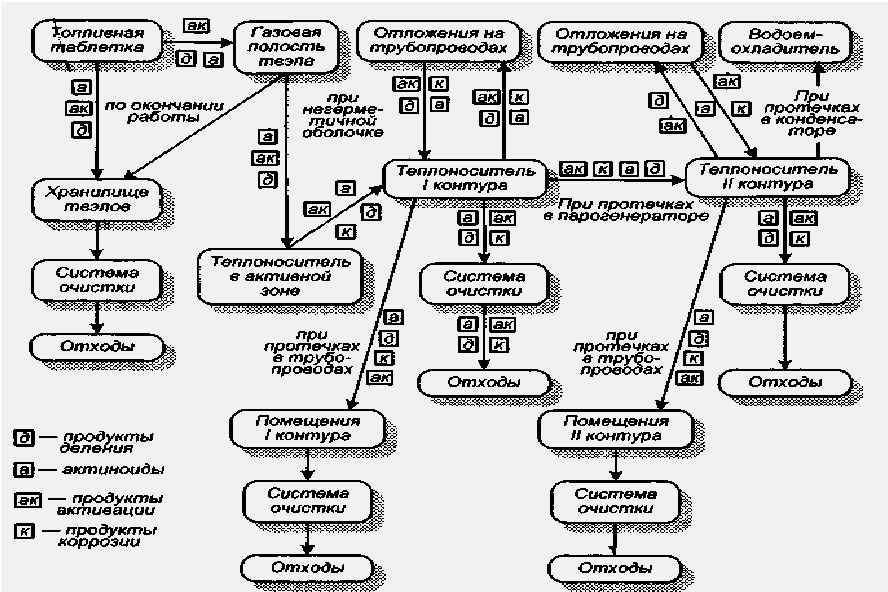
\includegraphics[width=16cm]{nuclides_spread}
	\captionsetup{justification=centering}
    \caption{Основные пути распространения радионуклидов на \ac{aes}.}
    \label{fig_nuclides_spread}
\end{figure}

Топливную таблетку в \ac{tvel}ах рассматривают как первый барьер распространения радиоактивных нуклидов в пределах 
активной зоны ядерного реактора. В результате реакции деления и захвата нейтронов в топливной таблетке накапливаются 
радионуклиды, изменяя состав, физико-химические и механические свойства топливной композиции. При температуре ниже 
1000 \degree C диоксид урана, который наиболее часто используется в качестве топлива в реакторах типа \ac{vver}, 
удерживает все радионуклиды, образующиеся в процессе работы реактора. При росте температуры ситуация существенно 
меняется, так как продукты захвата и деления становятся более подвижными \cite{leskin_vver}.

Между топливной таблеткой и оболочкой \ac{tvel}а присутствует небольшой зазор и газовая полость, предназначенные для 
накопления продуктов деления и активации, которым удалось покинуть пределы топливной таблетки.

Вторым барьером распространения радионуклидов является оболочка \ac{tvel}ов. В случае герметичной оболочки \ac{tvel}ов 
выход радионуклидов за пределы оболочки достаточно мал. В реальности, из за высоких тепловых и радиационных нагрузок и 
процессов коррозионно-усталостного типа оболочки теряют свою герметичность. Согласно \cite{kolpakov_tvel}, при 
эксплуатации ядерного реактора пределом безопасной эксплуатации по количеству и величине дефектов составляет 1 \% 
\ac{tvel}ов с дефектами типа газовой неплотности.

В случае разгерметизации топливной оболочки радионуклиды диффундируют через микротрещины в теплоноситель, находящийся 
в активной зоне реактора, который в дальнейшем переходит в первый контур реакторной установки. Более того, 
дополнительным источником радиоактивности в теплоносителе первого контура является его активация нейтронами. 

При эксплуатации \ac{aes} в нормальном режиме работы обеспечивается локализация радиоактивных продуктов деления, 
продуктов активации в реакторной установке и основных системах очистки от радиоактивных нуклидов. Парогенератор и 
трубопроводы первого и второго контуров не позволяют значительной части радионуклидов покинуть основные барьеры. Однако
при наличии микротрещин или протечек в парогенераторе радиоактивность первого контура может перейти в теплоноситель 
второго контура реакторной установки. В то же время, при протечках в трубопроводах первого или второго контура 
радионуклиды попадают в технические помещения, а далее загрязненный воздух через вентиляционные системы выбрасывается 
в атмосферу. Газообразные выбросы с \ac{aes} перед попаданием в атмосферу проходят сложную систему очистки, которая в 
свою очередь необходима для снижения активности выбросов, а далее попадают в окружающую среду через высокую трубу.

Помимо газообразных радиоактивных отходов при работе реактора выделяются жидкие и твердые отходы (рисунок 
\ref{fig_nuclides_spread2}). Твердыми радиоактивными отходами являются конструкционные материалы из активной зоны и 
первого контура, фильтры очистки установок, загрязненные инструменты, приборы и т.д. Твердые радиоактивные отходы после 
эксплуатации отправляются на захоронение. Жидкие радиоактивные отходы также образуются в результате эксплуатации 
\ac{aes}, в дальнейшем их очищают, разбавляют, фильтруют или концентрируют и хранят в специальных емкостях в жидком 
виде, однако при протечках в парогенераторе и конденсаторе радиоактивные отходы, мигрировавшие во второй контур 
реакторной установки, могут попасть в водоем-охладитель \cite{bekman_nuclear}. 

\begin{figure}[ht]
	\centering
	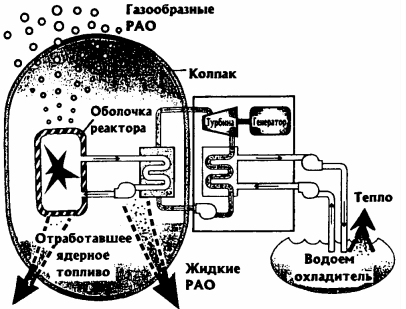
\includegraphics[width=10cm]{nuclides_spread2}
	\captionsetup{justification=centering}
    \caption{Схема образования газообразных, жидких и твердых отходов от \ac{aes} \cite{bekman_nuclear}.}
    \label{fig_nuclides_spread2}
\end{figure}